\subsection{Fichier de tests}
	La structure utilisée dans le fichier de tests est la suivante:
	\begin{itemize}
		\item Chaque ligne ne peut excéder 100 caractères,
		\item Le premier caractère de chaque ligne peut-être:
		\begin{itemize}
			\item \texttt{\#}: Permet d'afficher le texte présent sur la ligne, après le caractère.
			\item \texttt{p}: Permet de lancer le test de la pile. Nécessite un argument: le nombre d'éléments, donné sur la même ligne.
			\item \texttt{t}: Permet de lancer la fonction \texttt{truc} en version itérative. Prend deux arguments positifs, strictement pour le second. Le premier correspond à S, le second à I.
			\item \texttt{T}: Idem pour la version récursive.
			\item Tout autre caractère ou ligne vide affichera une ligne vide.
		\end{itemize}
	\end{itemize}
	Le programme est exécuté avec le fichier \texttt{tests/test}:
	\inputminted[frame=single,label=Test]{text}{../tests/test}
	On obtient alors le résultat suivant: 
	\inputminted[frame=single,label=Resultat]{text}{../tests/resultat_test}

\subsection{Tests de la pile}
	Avec l'outil \texttt{ddd} nous présentons ici l'utilisation de la pile dans les tests \no 3 et 4 du fichier de tests. 
	\begin{figure}[H]
		\begin{subfigure}[c]{0.33\textwidth}
			\centering
	  	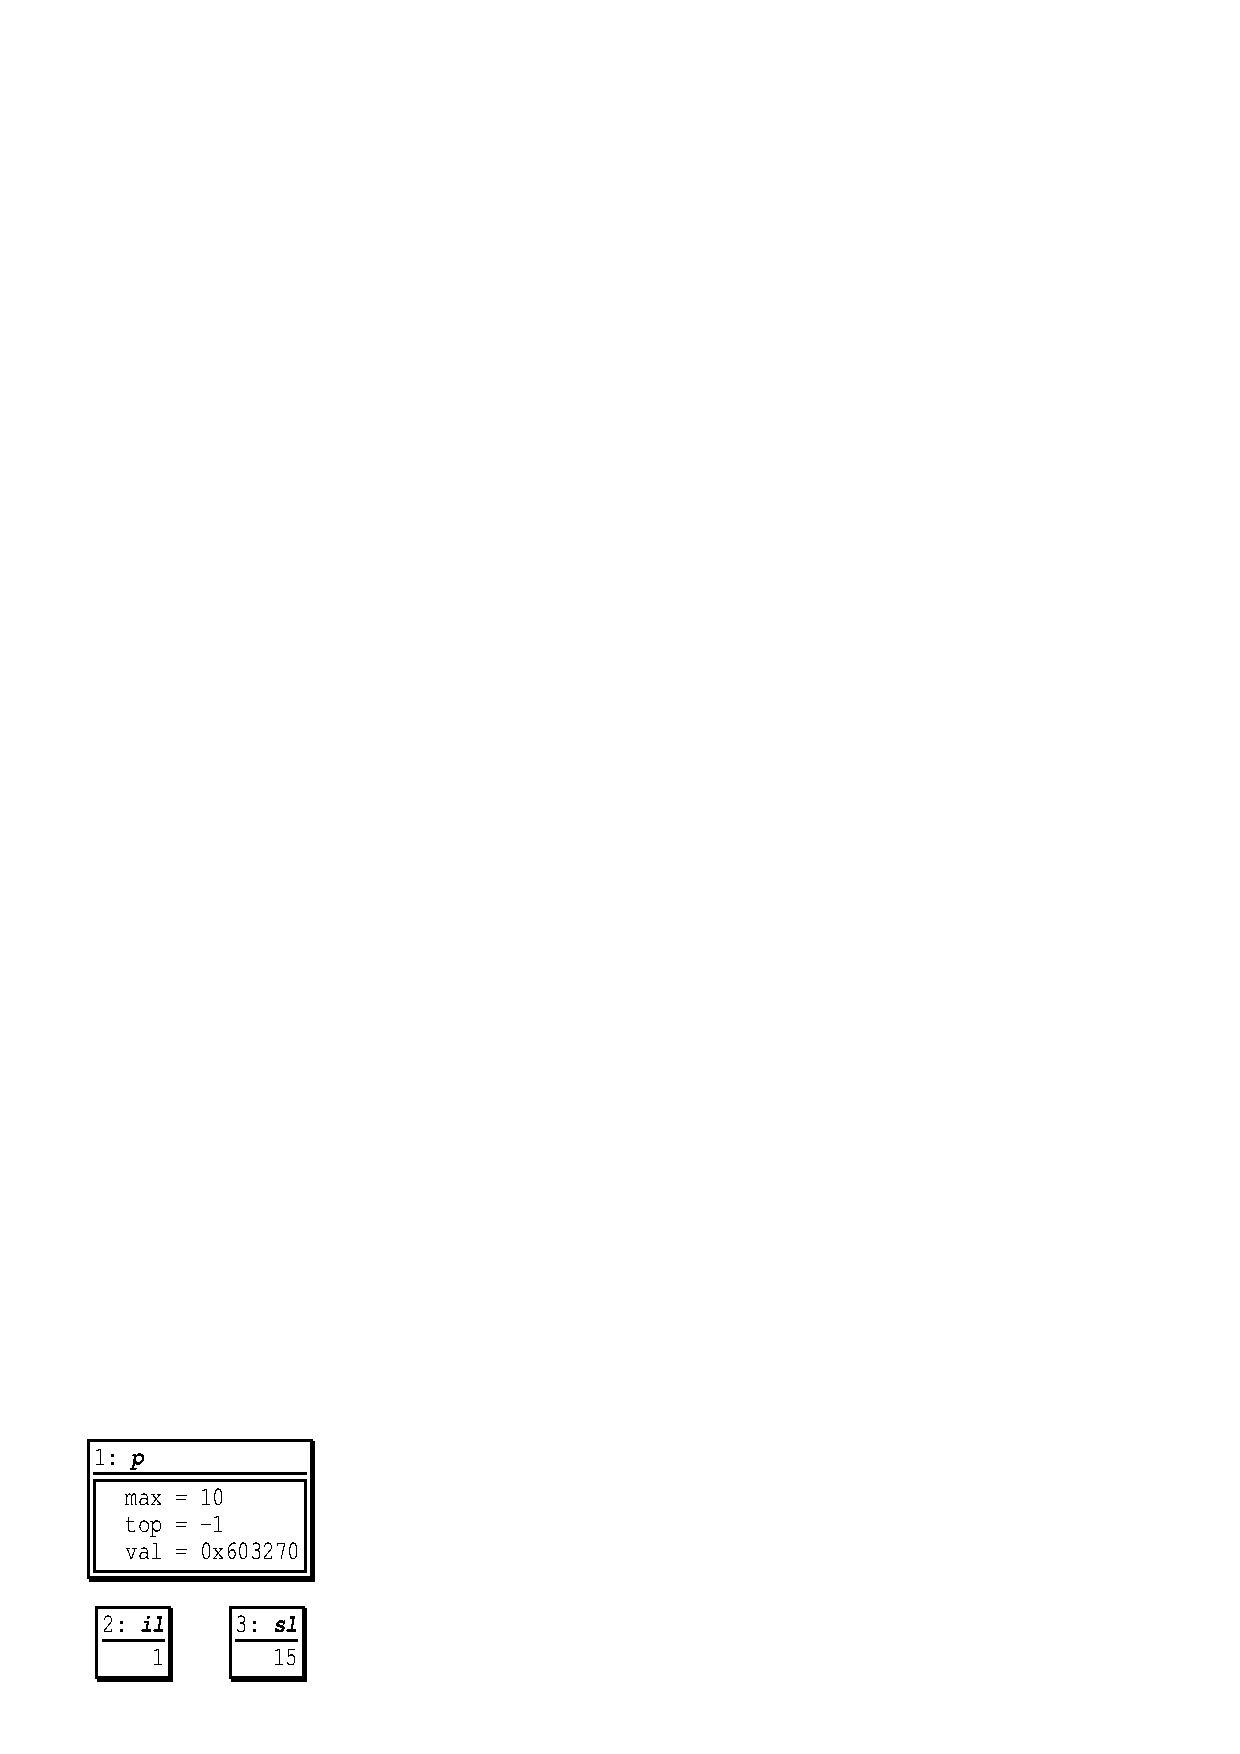
\includegraphics[width=3cm,clip=true,trim=1cm 1cm 15cm 24cm]{../tests/ddd_graph/ddd_3_0}
			\subcaption{Début}
		\end{subfigure}
		\begin{subfigure}[c]{0.33\textwidth}
			\centering
			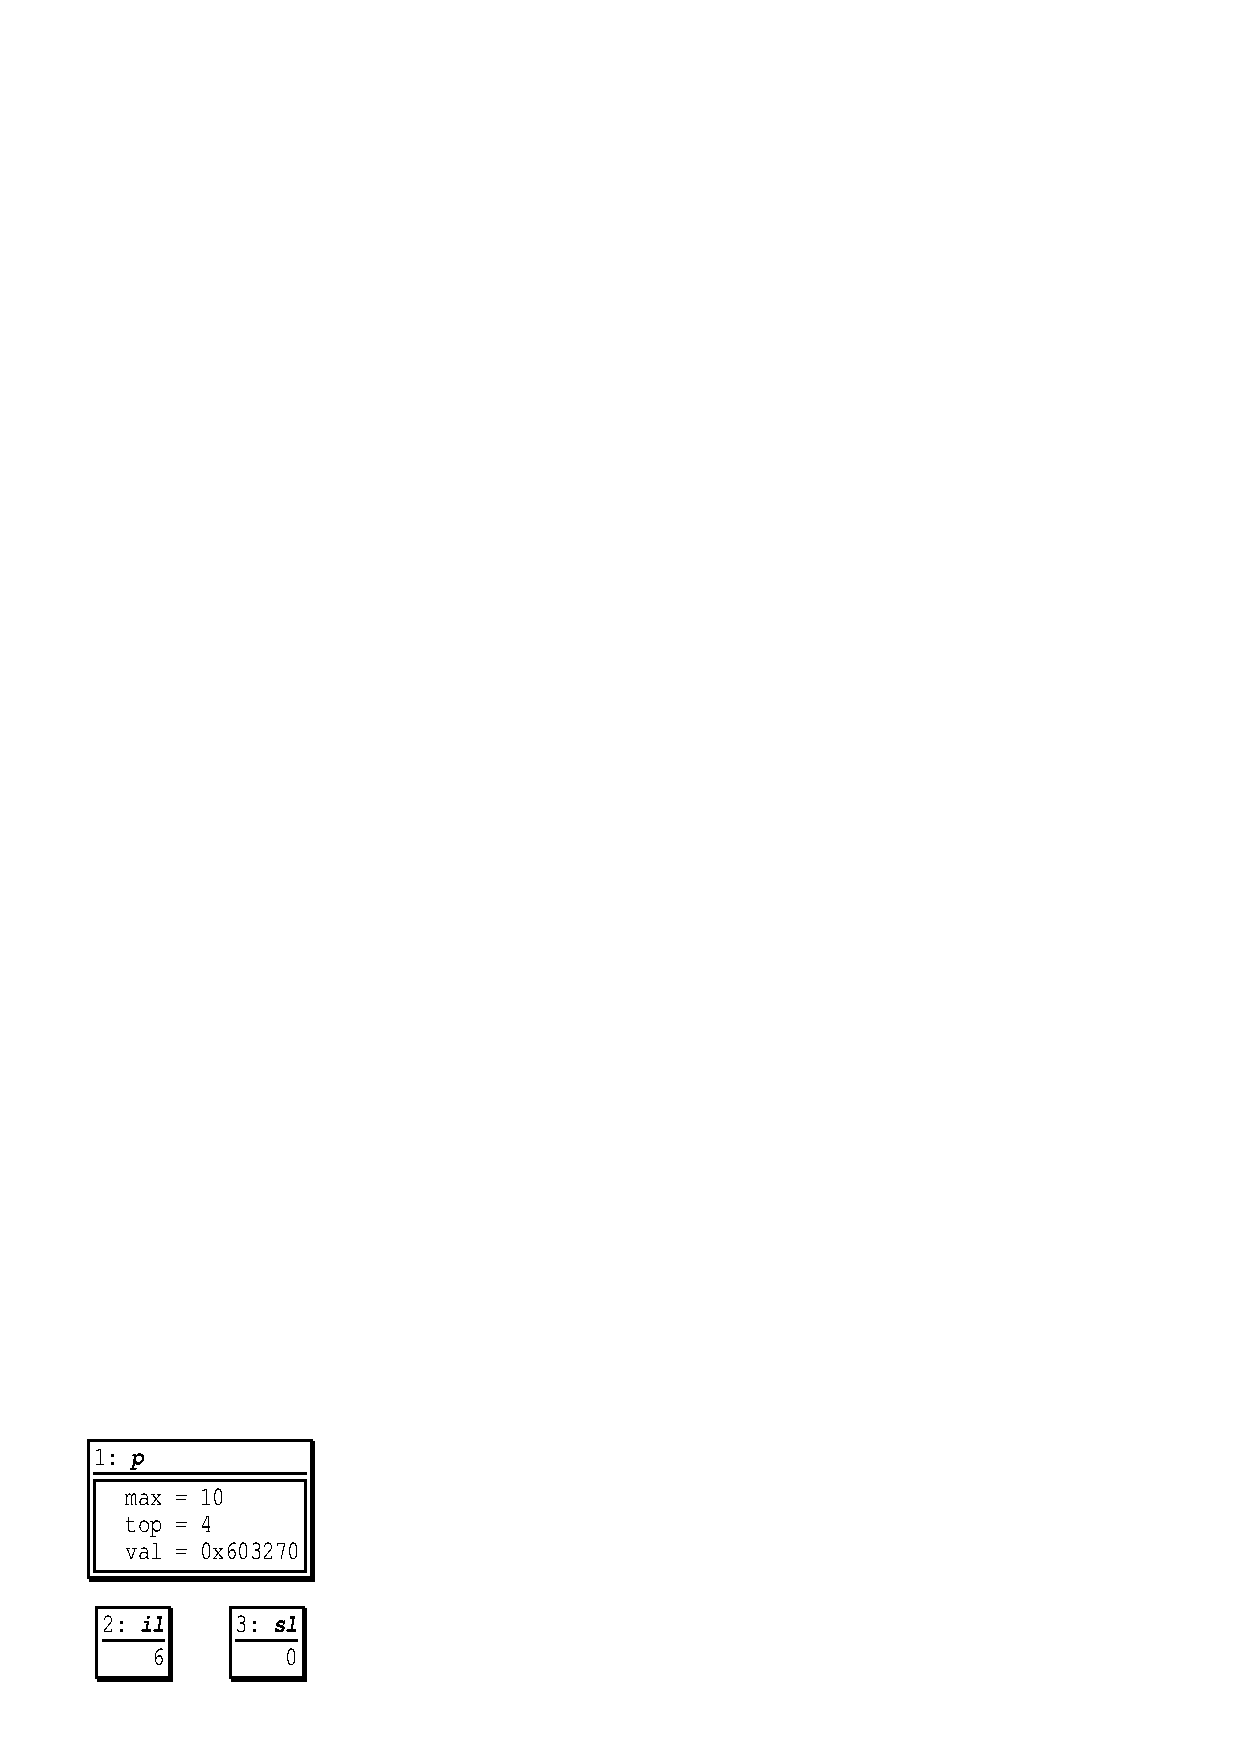
\includegraphics[width=3cm,clip=true,trim=1cm 1cm 15cm 24cm]{../tests/ddd_graph/ddd_3_1}
			\subcaption{Après avoir empilé 1, 2, 3, 4 et 5}
		\end{subfigure}
		\begin{subfigure}[c]{0.33\textwidth}
			\centering
	  	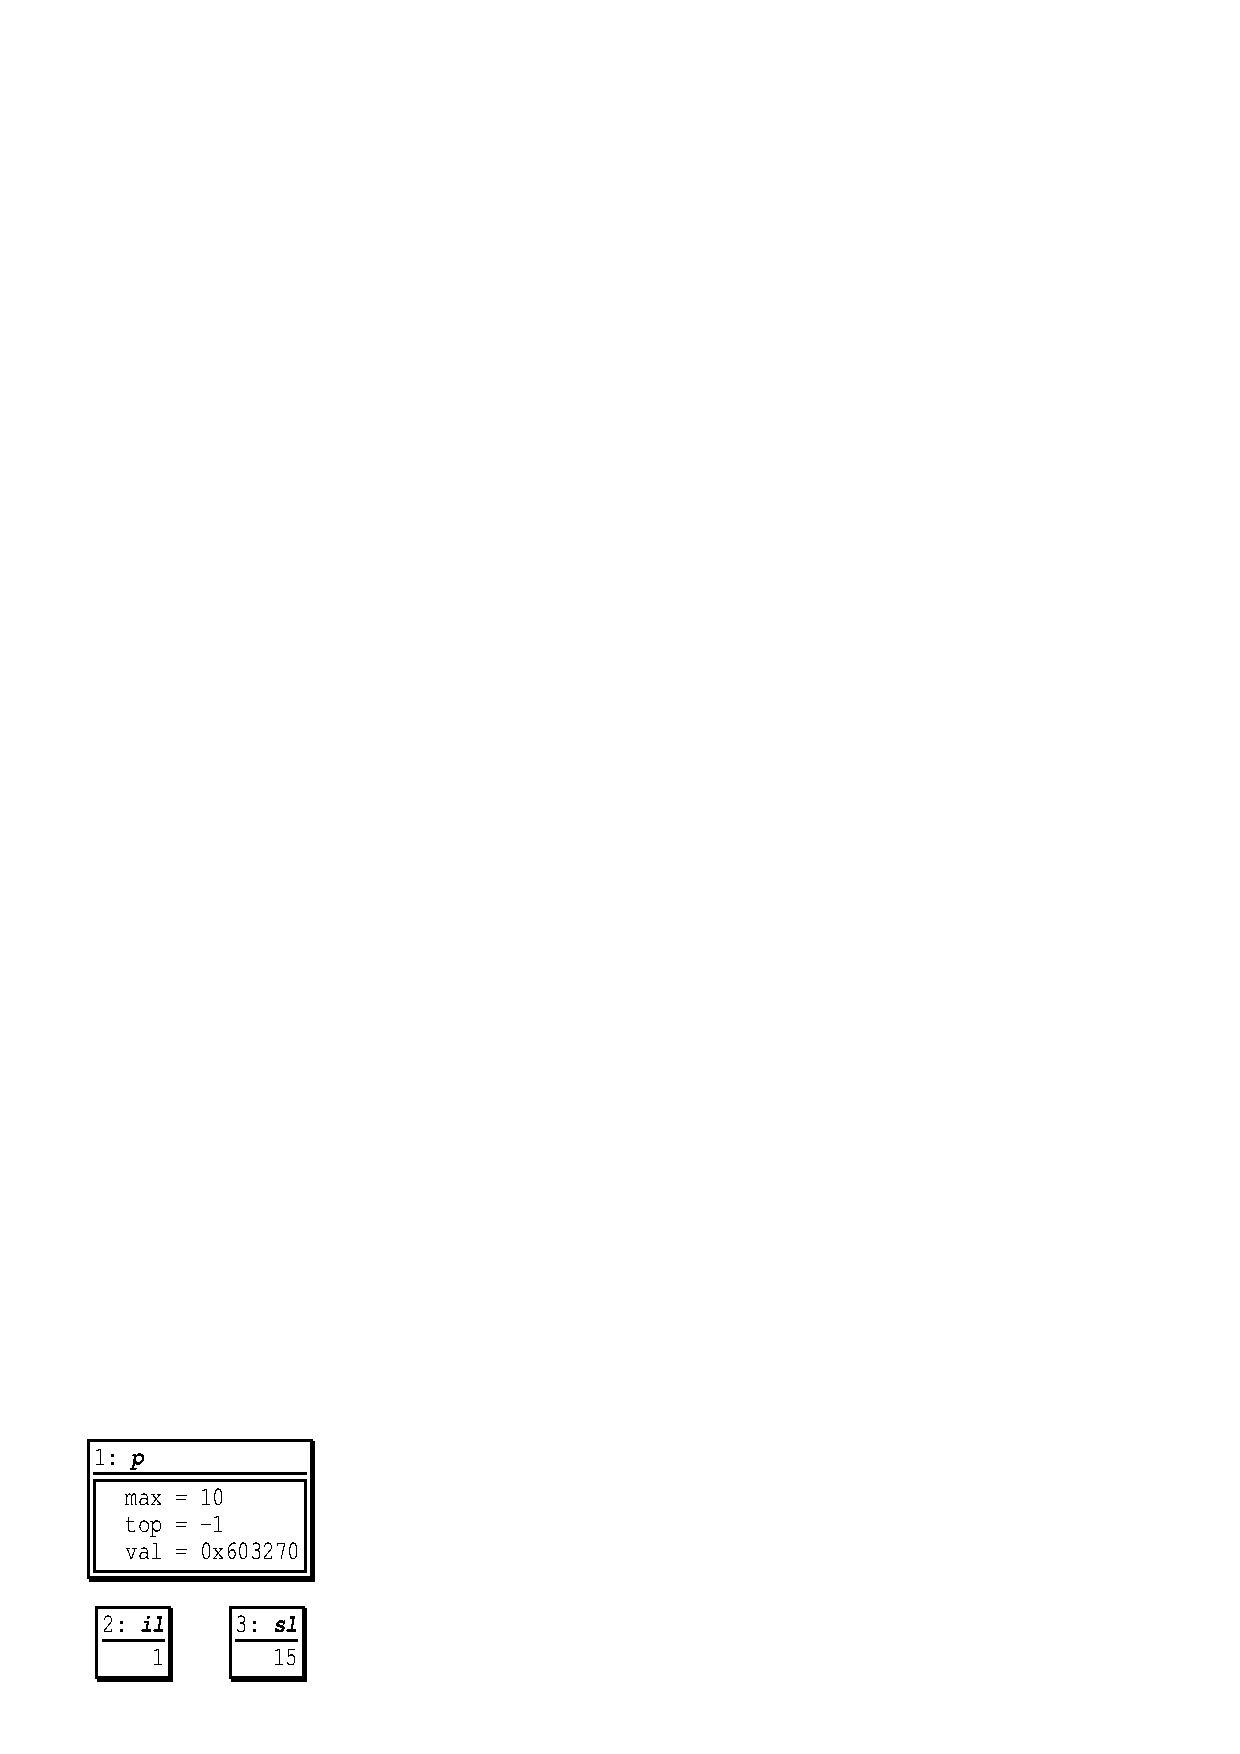
\includegraphics[width=3cm,clip=true,trim=1cm 1cm 15cm 24cm]{../tests/ddd_graph/ddd_3_2}
			\subcaption{Fin, après avoir dépilé 5, 4, 3, 2 et 1}
		\end{subfigure}
	  \caption{Test n°3 -- Aperçu des informations de la pile dans \texttt{ddd}}
	\end{figure}
	\begin{figure}[H]
		\begin{subfigure}[c]{0.33\textwidth}
			\centering
			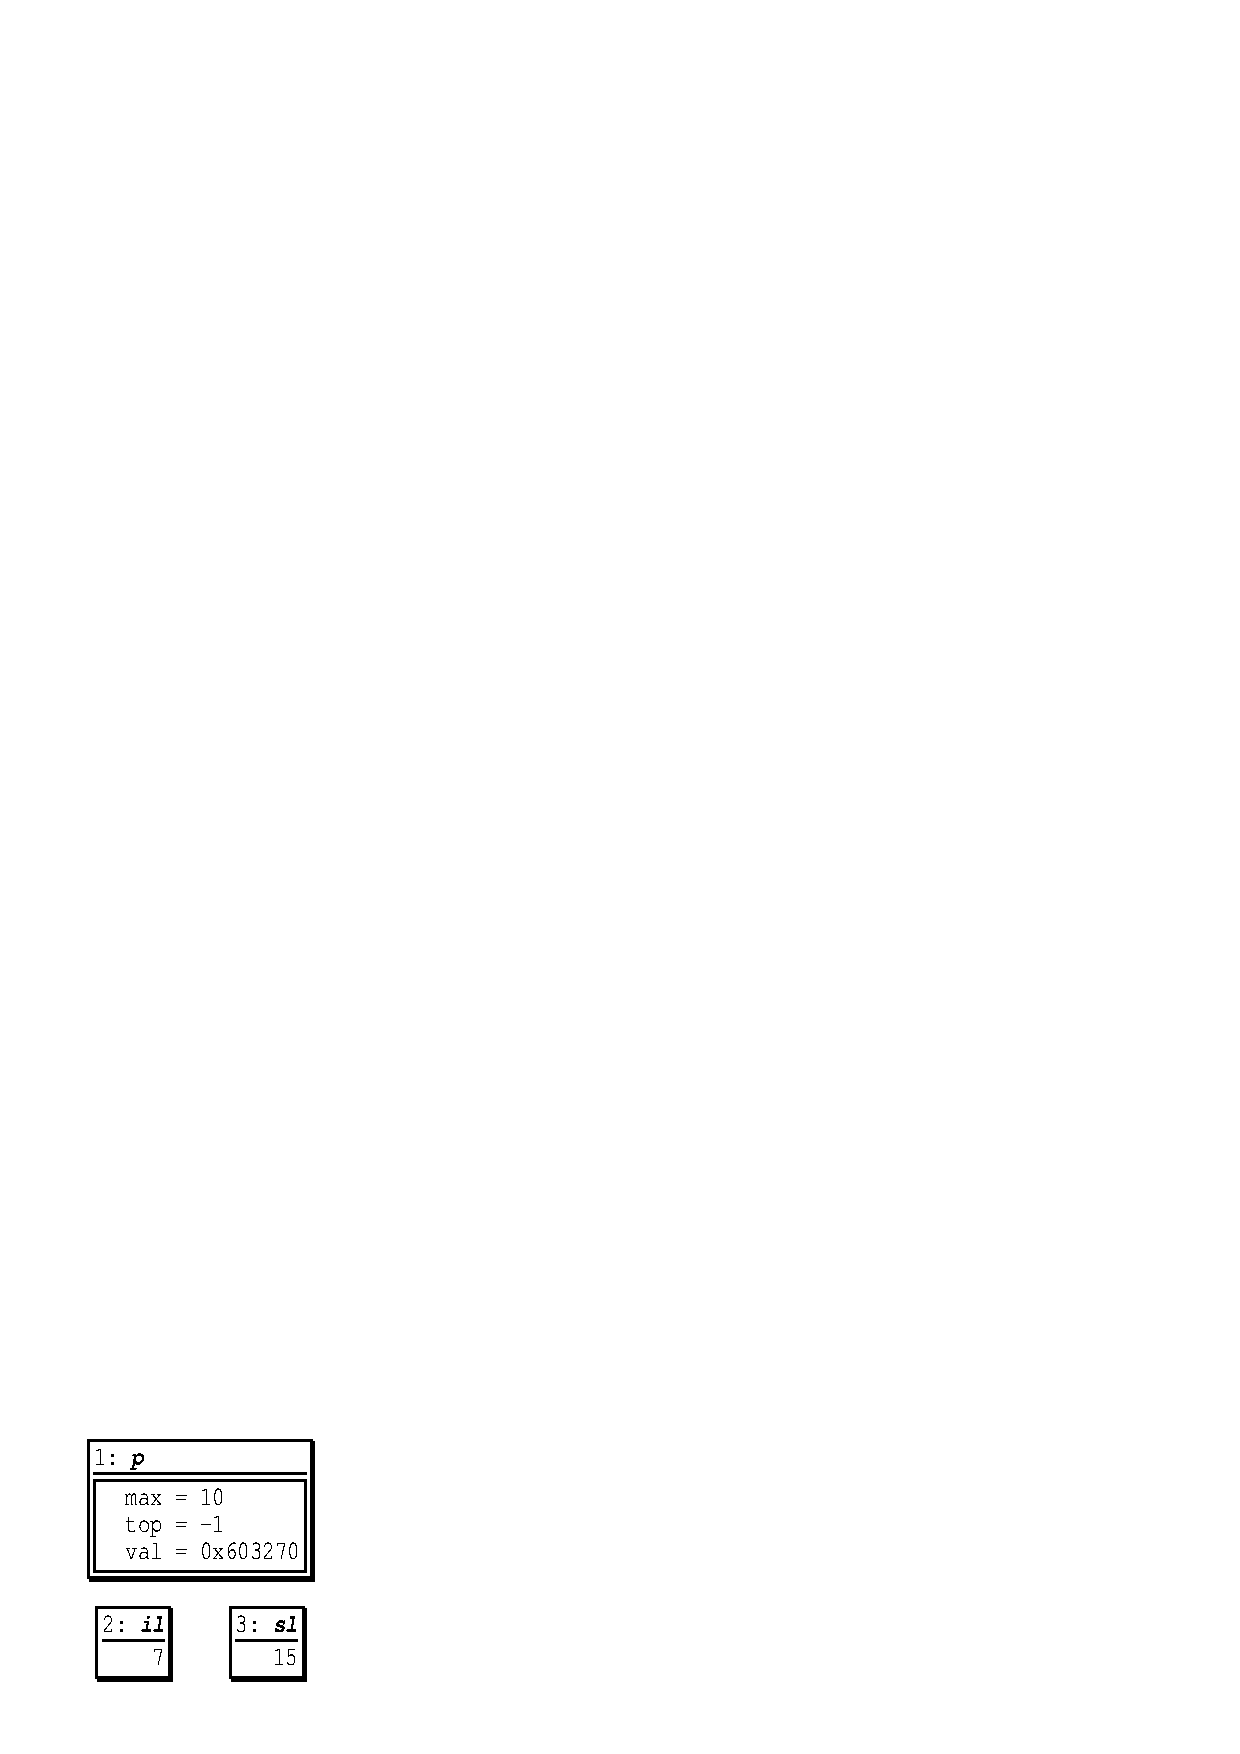
\includegraphics[width=3cm,clip=true,trim=1cm 1cm 15cm 24cm]{../tests/ddd_graph/ddd_4_0}
			\subcaption{Début}
		\end{subfigure}
		\begin{subfigure}[c]{0.33\textwidth}
			\centering
			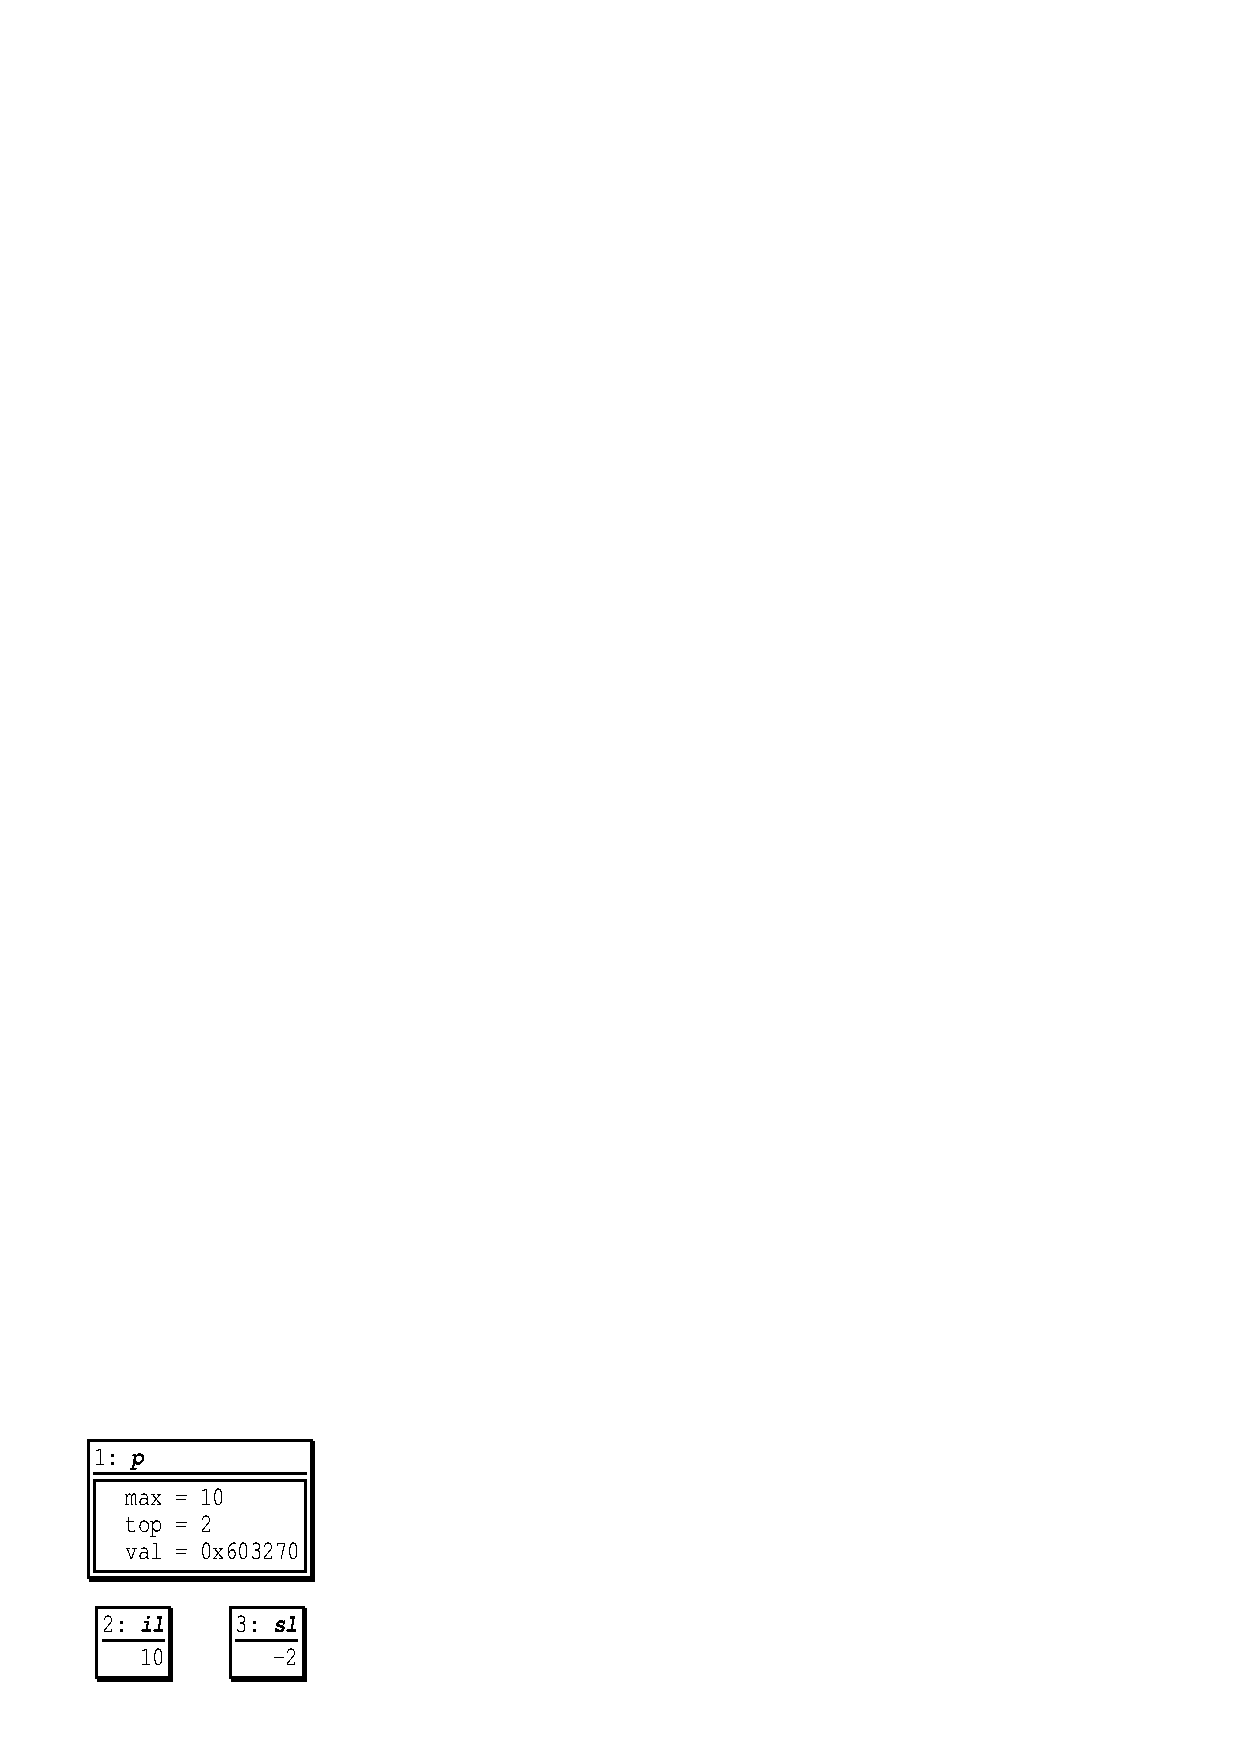
\includegraphics[width=3cm,clip=true,trim=1cm 1cm 15cm 24cm]{../tests/ddd_graph/ddd_4_1}
			\subcaption{Après avoir empilé 7, 8 et 9}
		\end{subfigure}
		\begin{subfigure}[c]{0.33\textwidth}
			\centering
			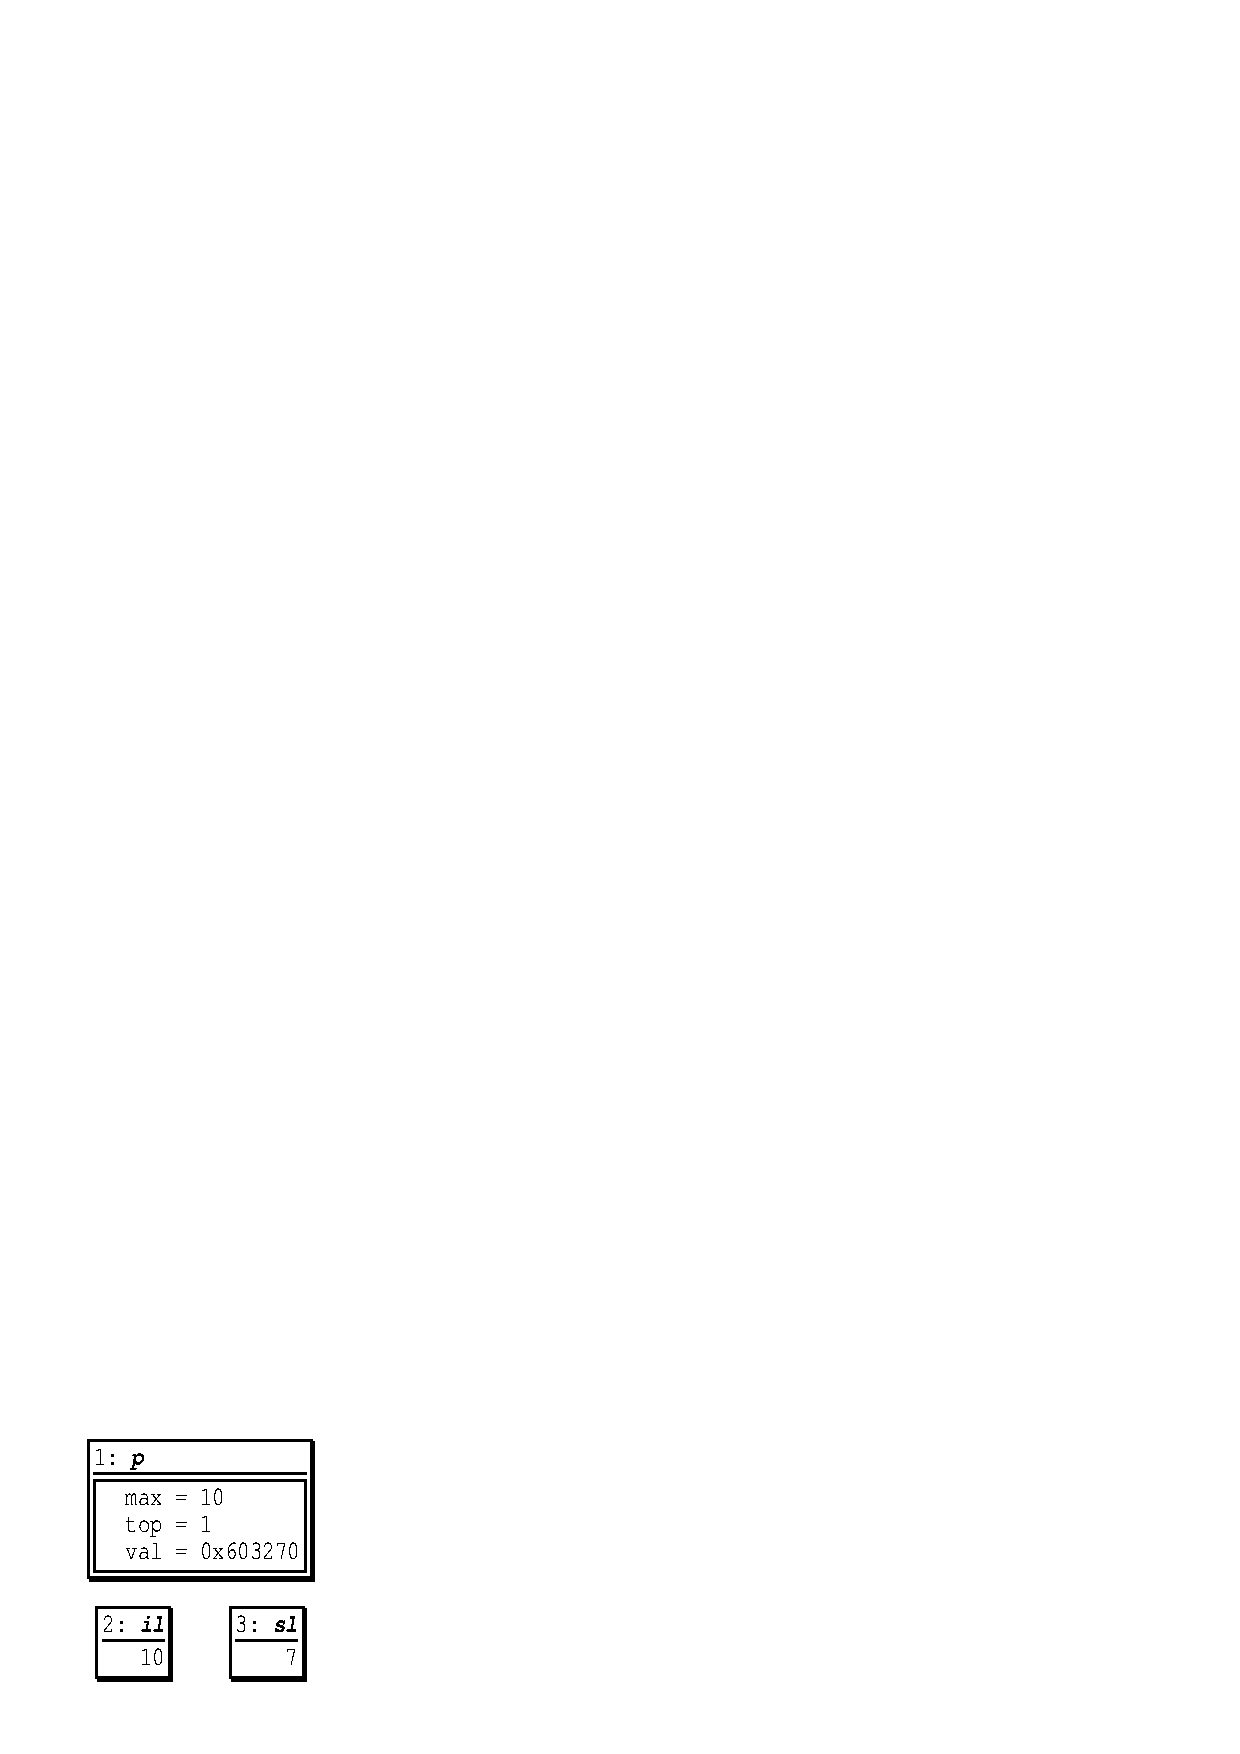
\includegraphics[width=3cm,clip=true,trim=1cm 1cm 15cm 24cm]{../tests/ddd_graph/ddd_4_2}
			\subcaption{Après avoir dépilé 9}
		\end{subfigure}
		\begin{subfigure}[c]{0.33\textwidth}
			\centering
			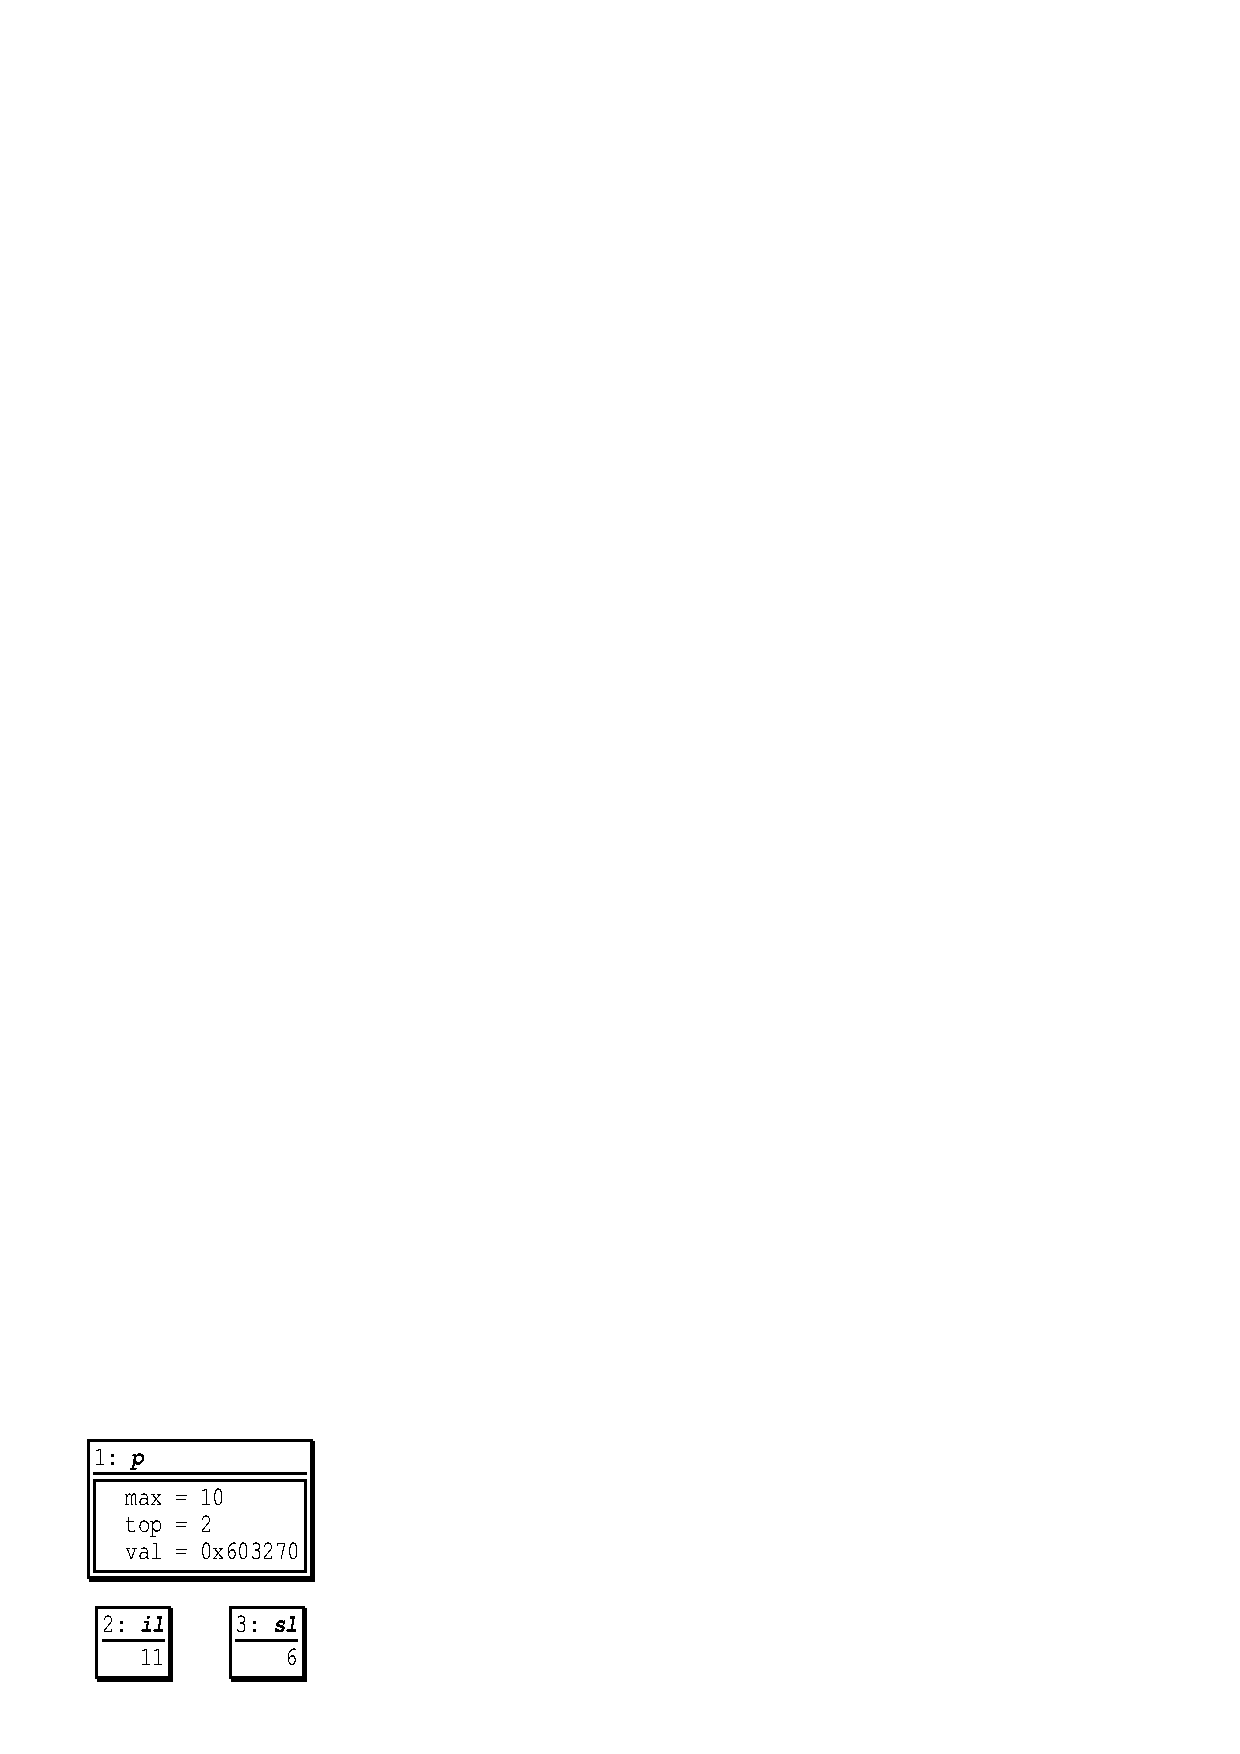
\includegraphics[width=3cm,clip=true,trim=1cm 1cm 15cm 24cm]{../tests/ddd_graph/ddd_4_3}
			\subcaption{Après avoir empilé 10}
		\end{subfigure}
		\begin{subfigure}[c]{0.33\textwidth}
			\centering
			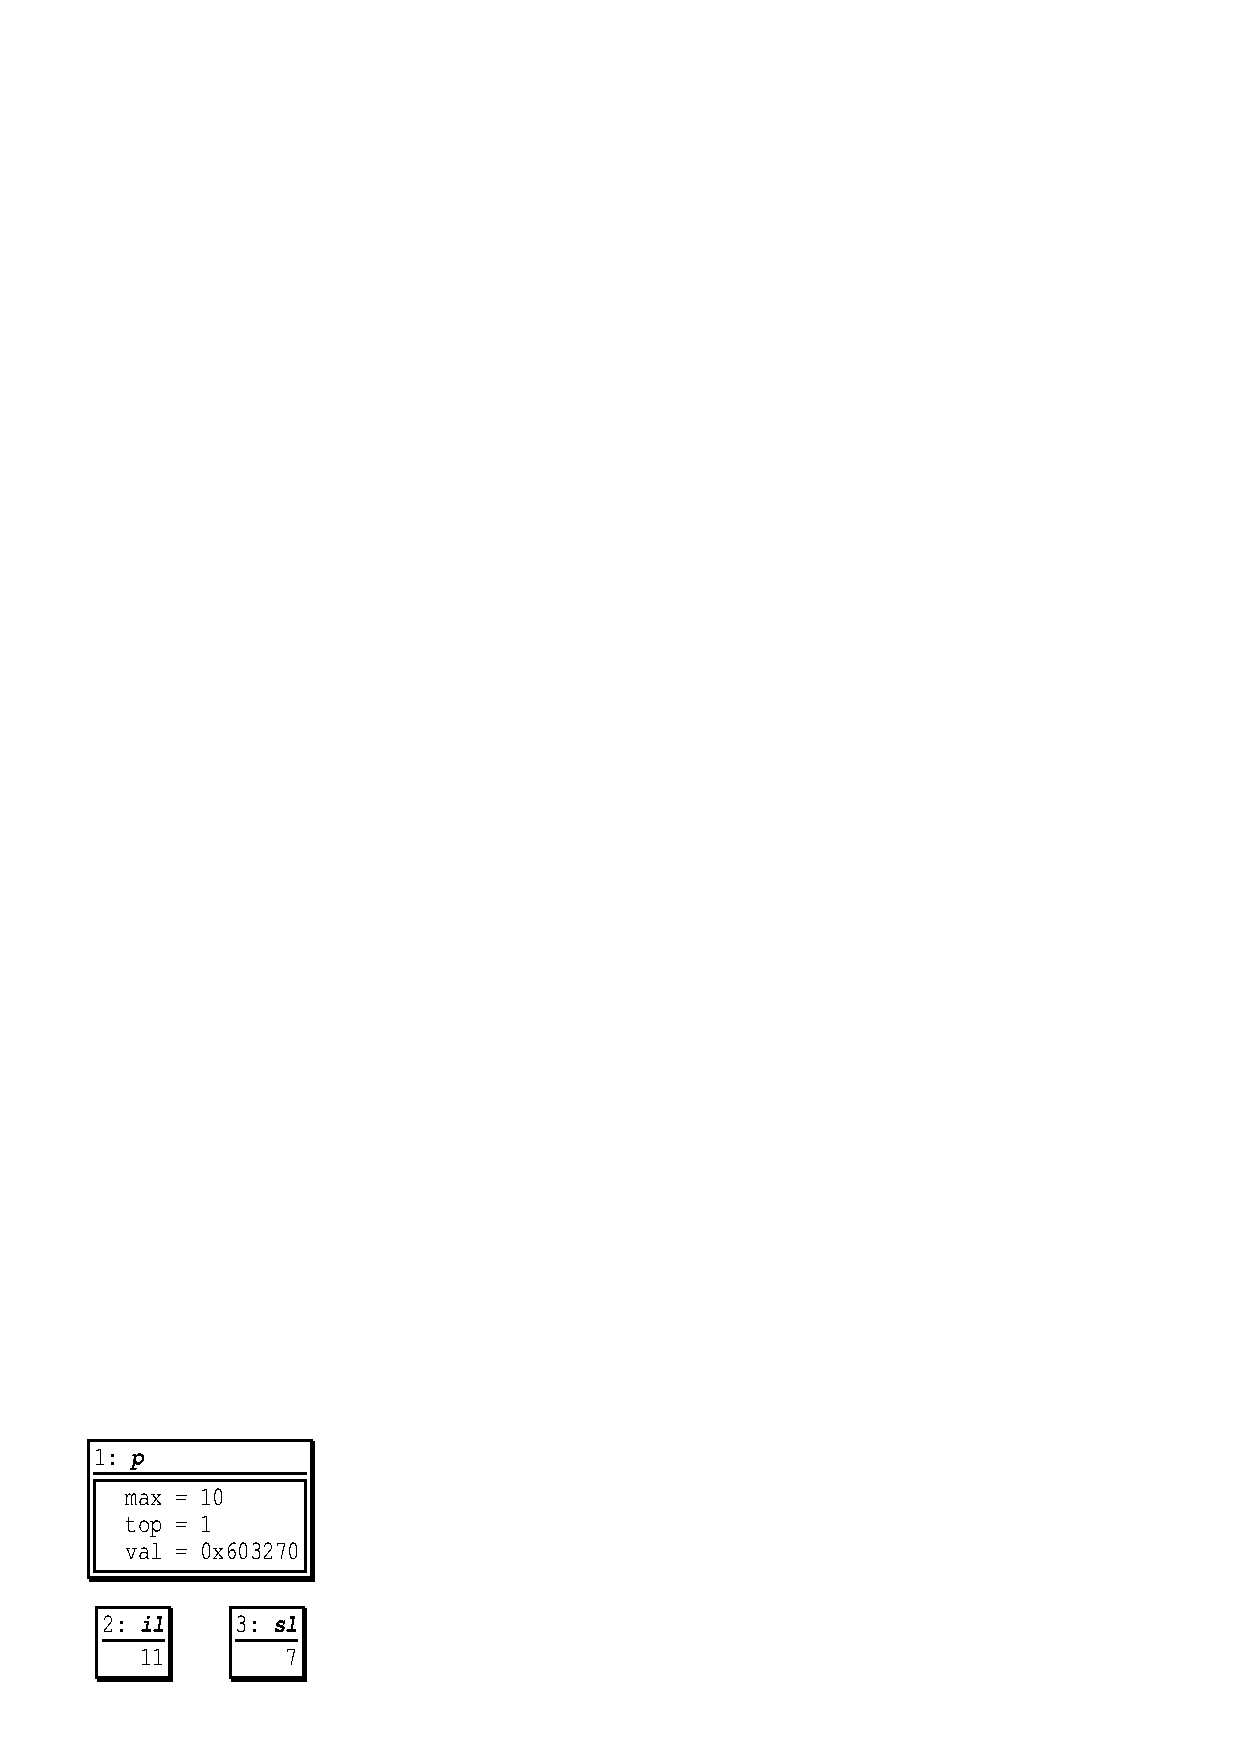
\includegraphics[width=3cm,clip=true,trim=1cm 1cm 15cm 24cm]{../tests/ddd_graph/ddd_4_4}
			\subcaption{Après avoir dépilé 10}
		\end{subfigure}
		\begin{subfigure}[c]{0.33\textwidth}
			\centering
			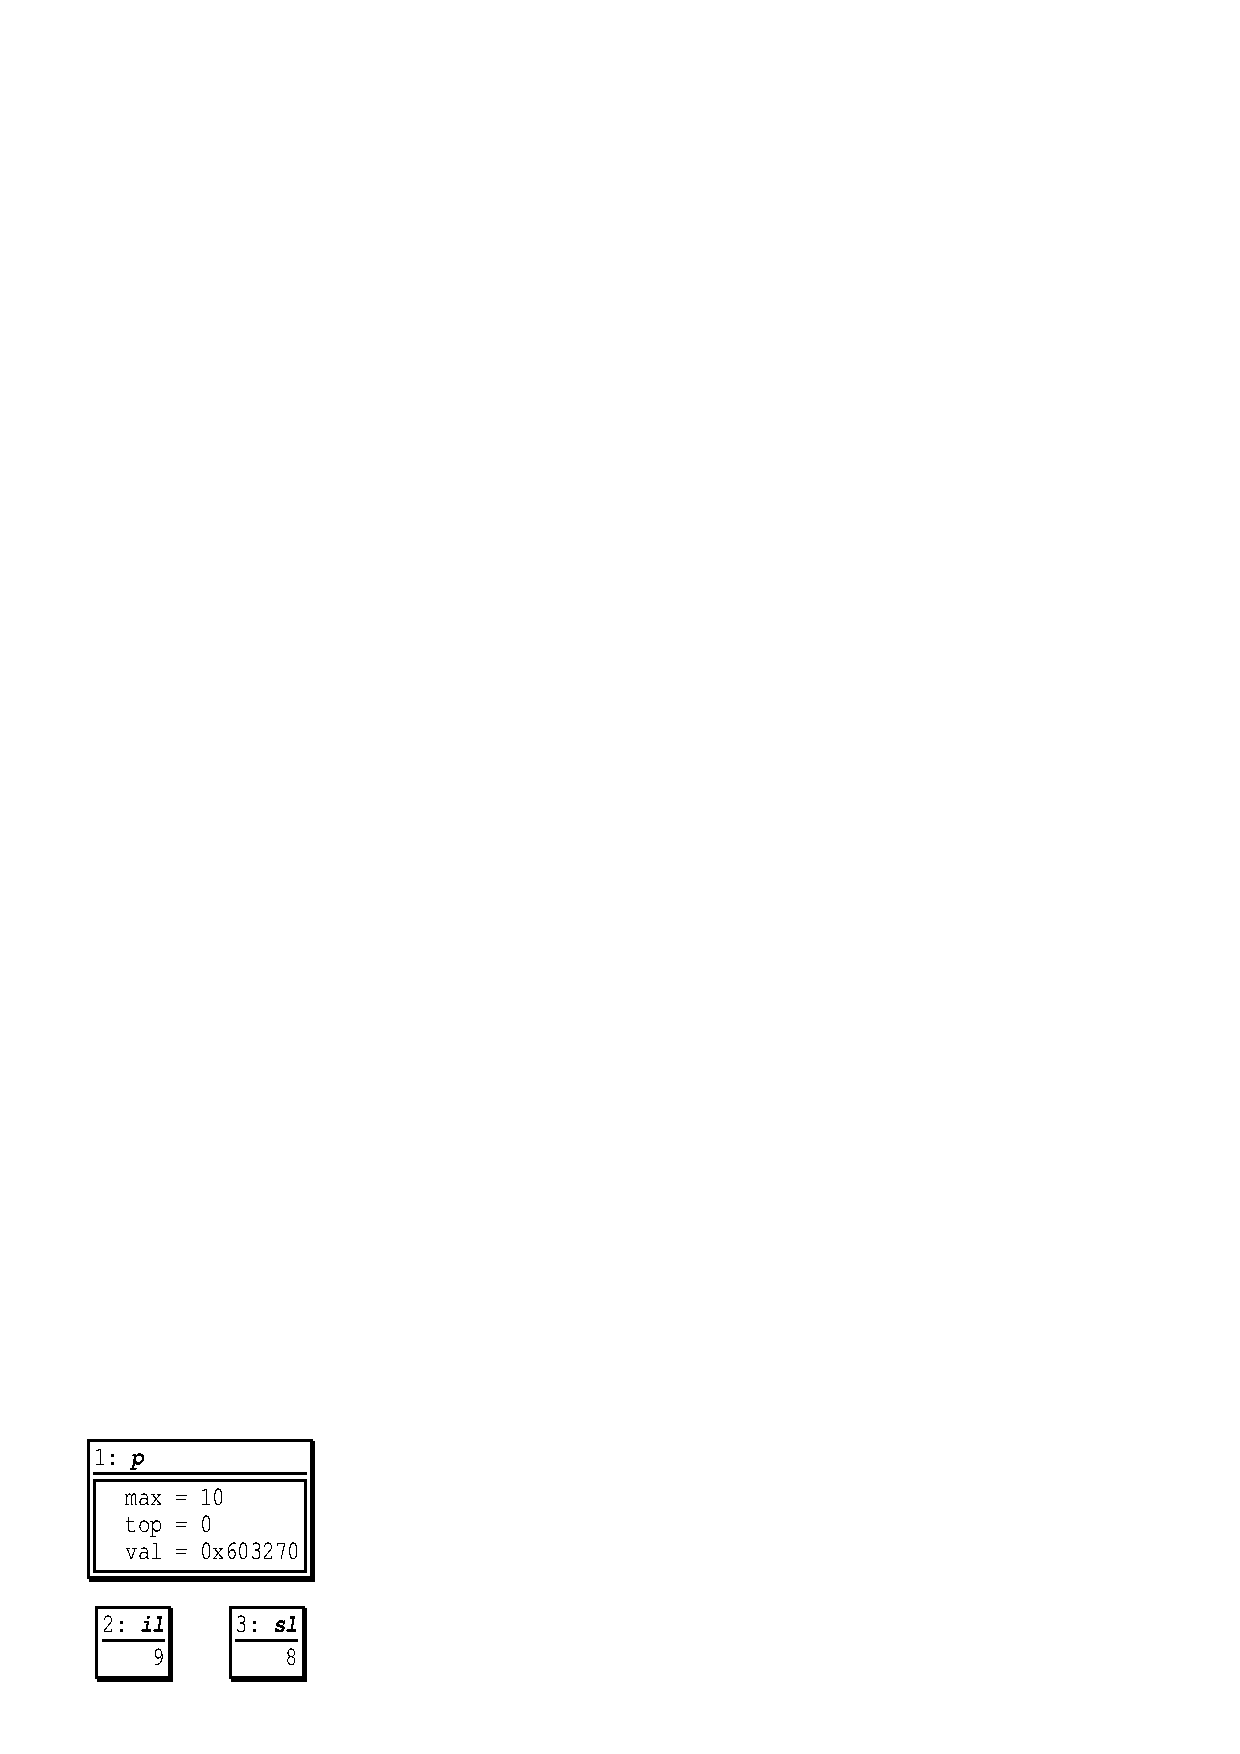
\includegraphics[width=3cm,clip=true,trim=1cm 1cm 15cm 24cm]{../tests/ddd_graph/ddd_4_6}
			\subcaption{Après avoir dépilé 8}
		\end{subfigure}
		\begin{subfigure}[c]{0.33\textwidth}
			\centering
			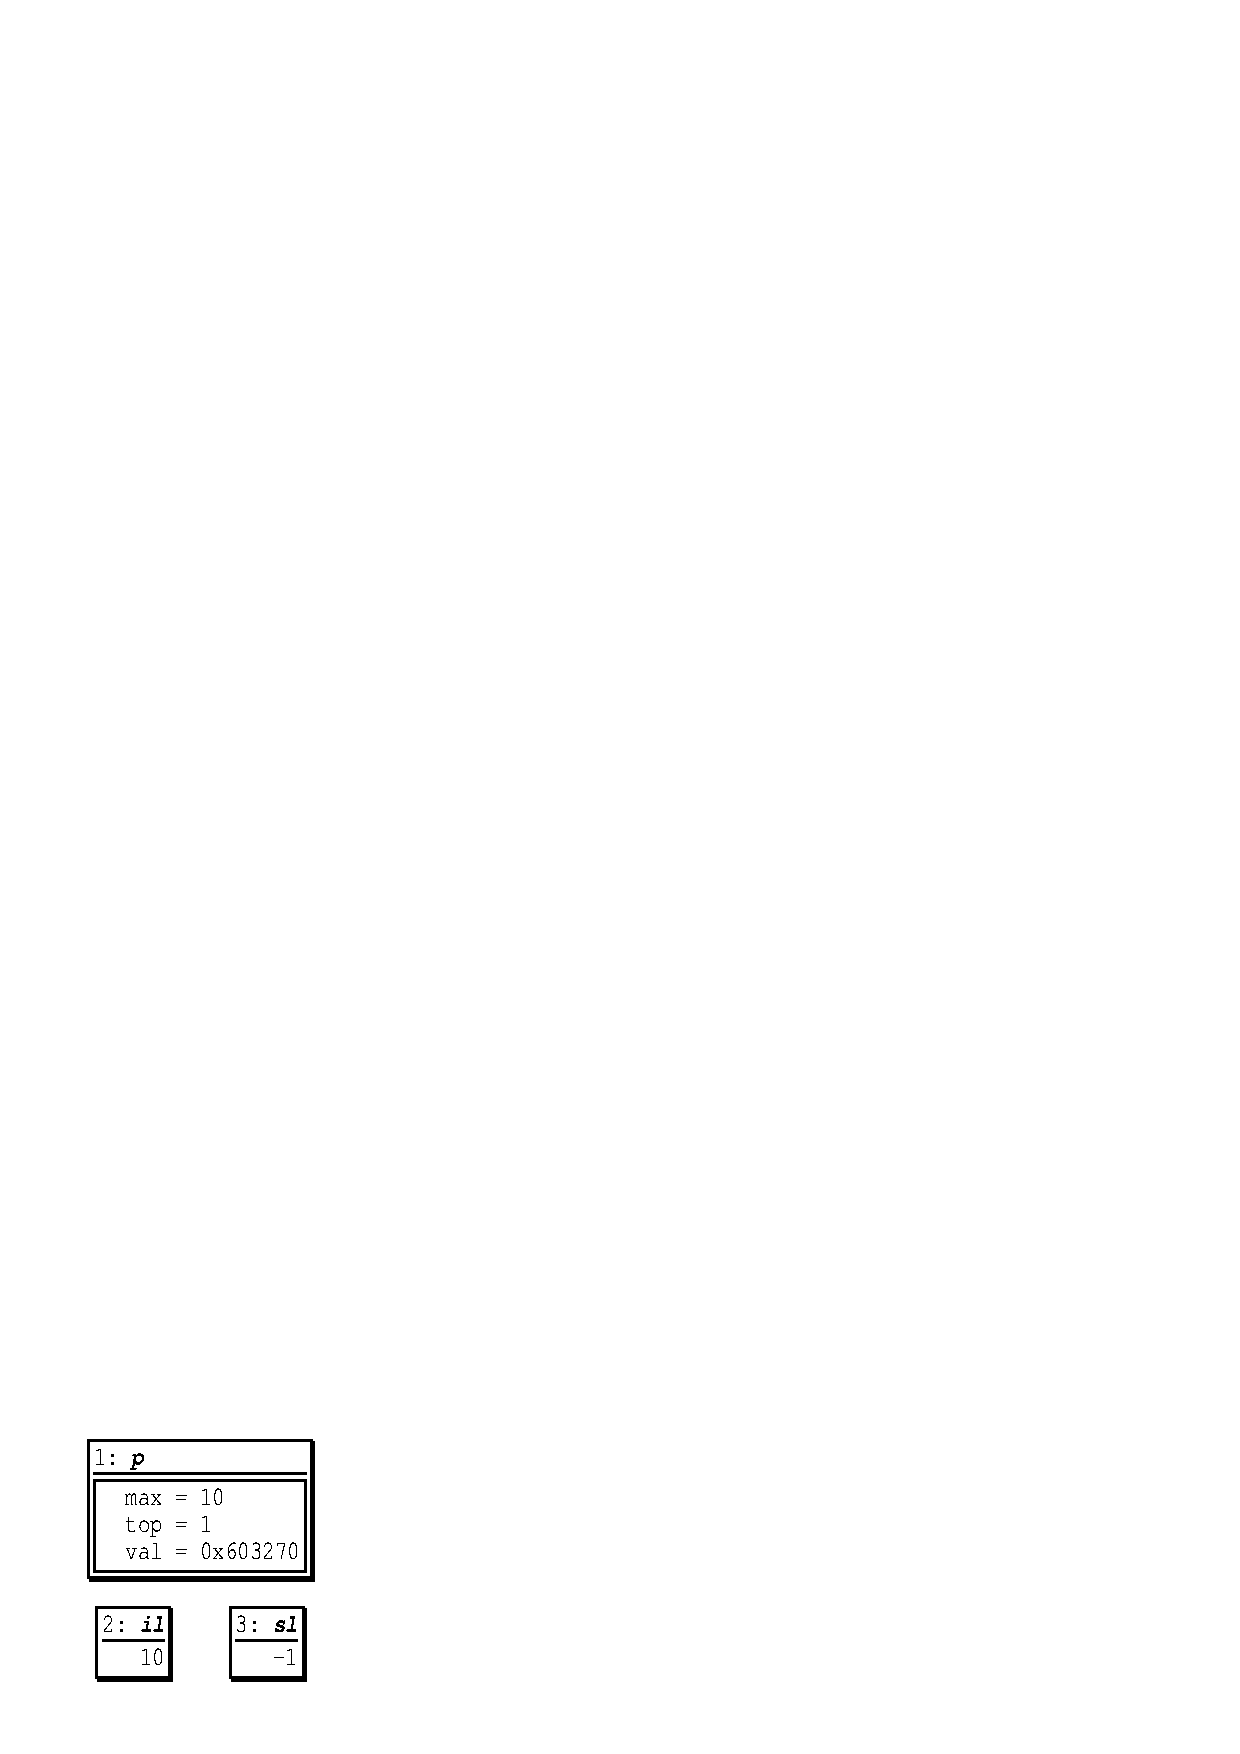
\includegraphics[width=3cm,clip=true,trim=1cm 1cm 15cm 24cm]{../tests/ddd_graph/ddd_4_7}
			\subcaption{Après avoir empilé 9}
		\end{subfigure}
		\begin{subfigure}[c]{0.33\textwidth}
			\centering
			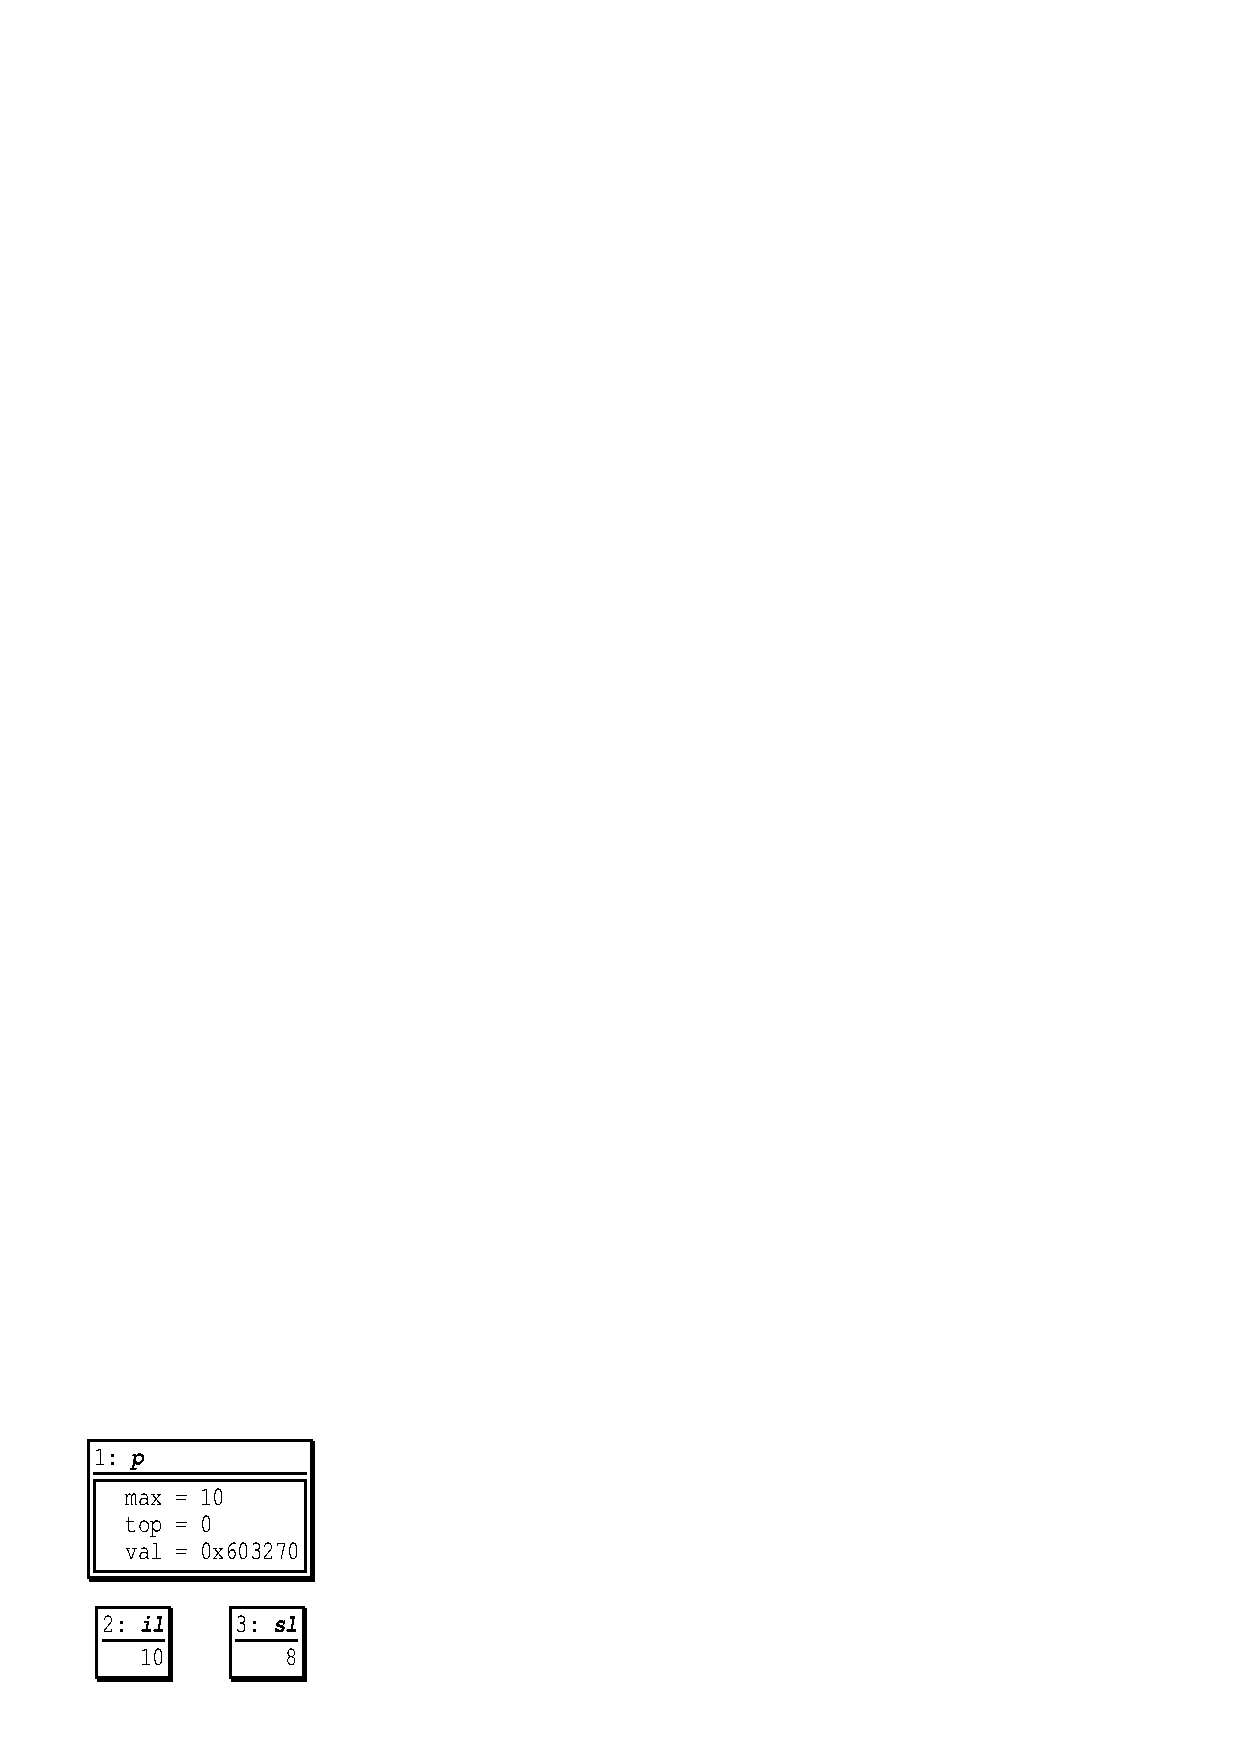
\includegraphics[width=3cm,clip=true,trim=1cm 1cm 15cm 24cm]{../tests/ddd_graph/ddd_4_8}
			\subcaption{Après avoir dépilé 9}
		\end{subfigure}
		\begin{subfigure}[c]{0.33\textwidth}
			\centering
			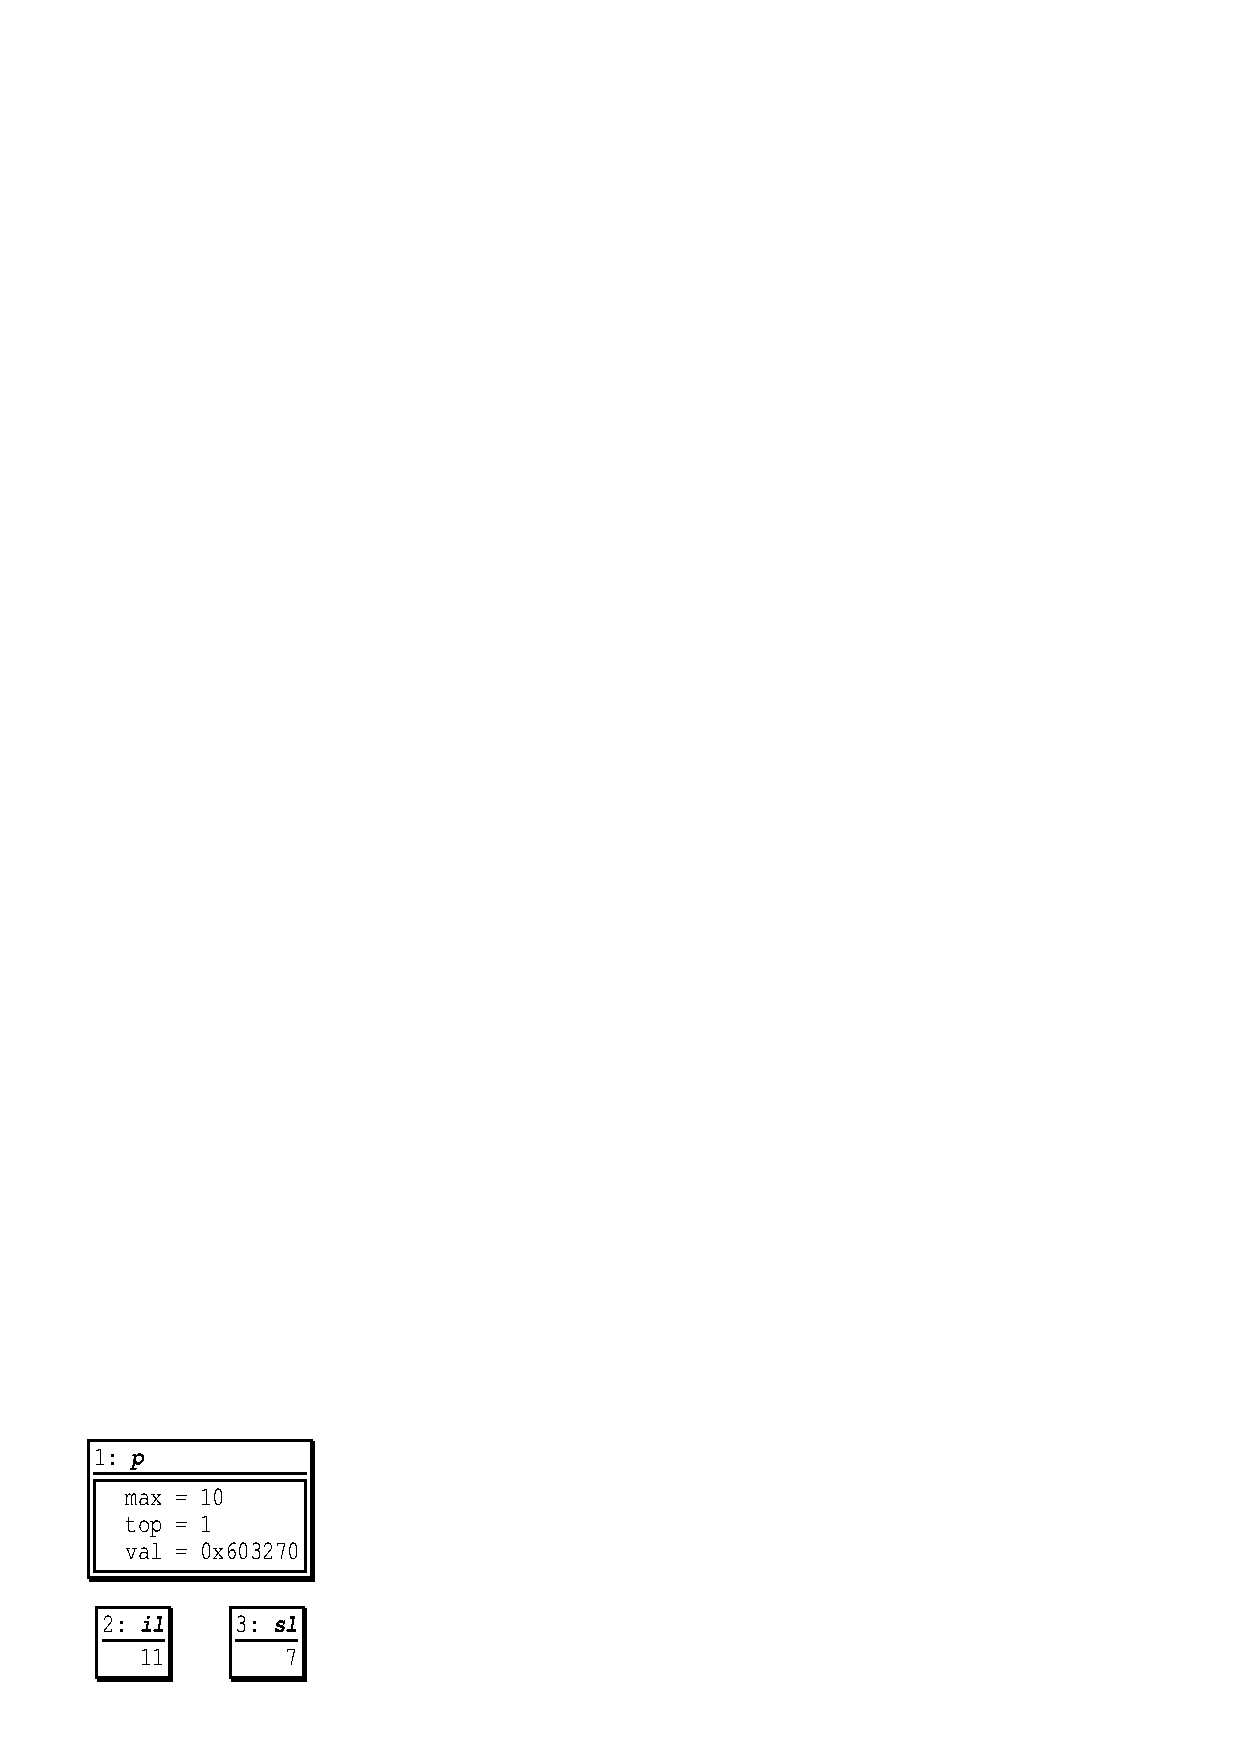
\includegraphics[width=3cm,clip=true,trim=1cm 1cm 15cm 24cm]{../tests/ddd_graph/ddd_4_9}
			\subcaption{Après avoir empilé 10}
		\end{subfigure}
		\begin{subfigure}[c]{0.33\textwidth}
			\centering
			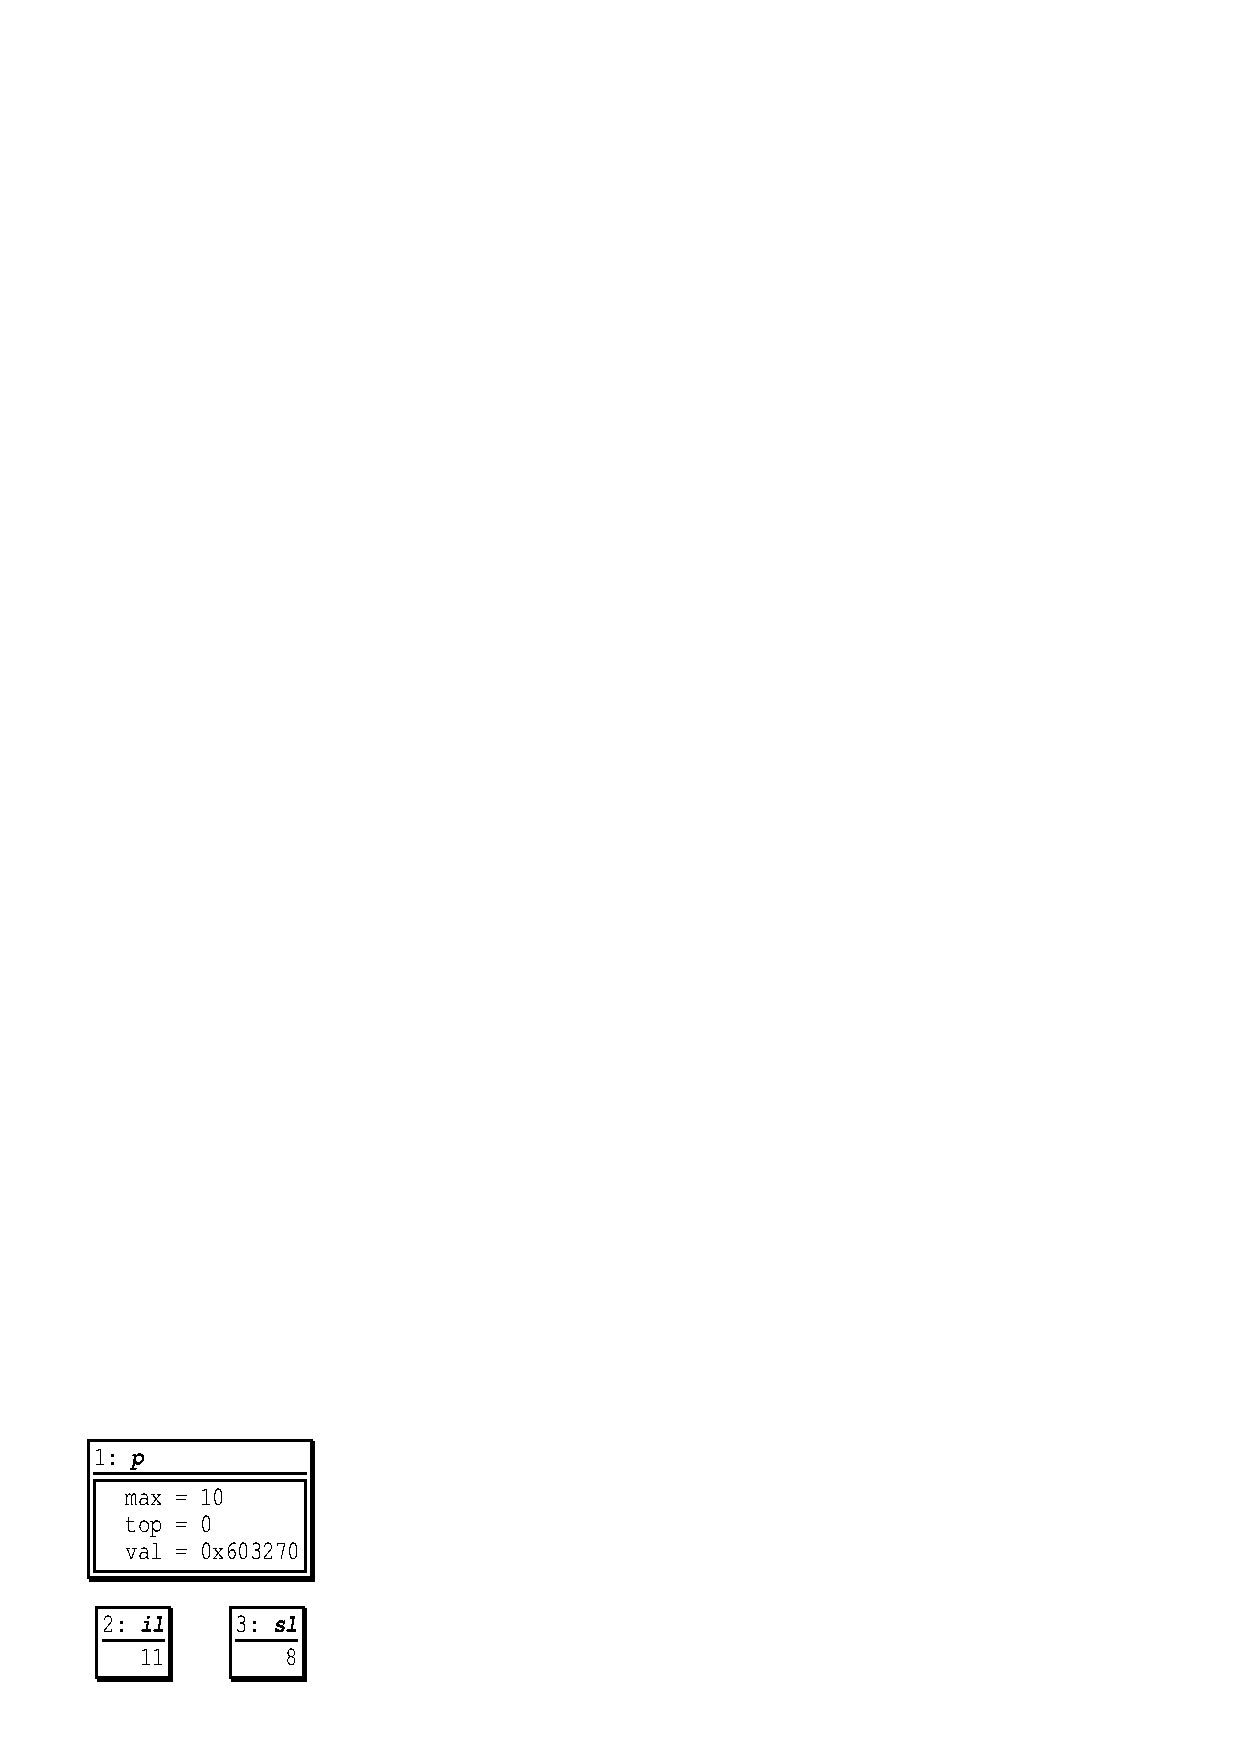
\includegraphics[width=3cm,clip=true,trim=1cm 1cm 15cm 24cm]{../tests/ddd_graph/ddd_4_10}
			\subcaption{Après avoir dépilé 10}
		\end{subfigure}
		\begin{subfigure}[c]{0.33\textwidth}
			\centering
			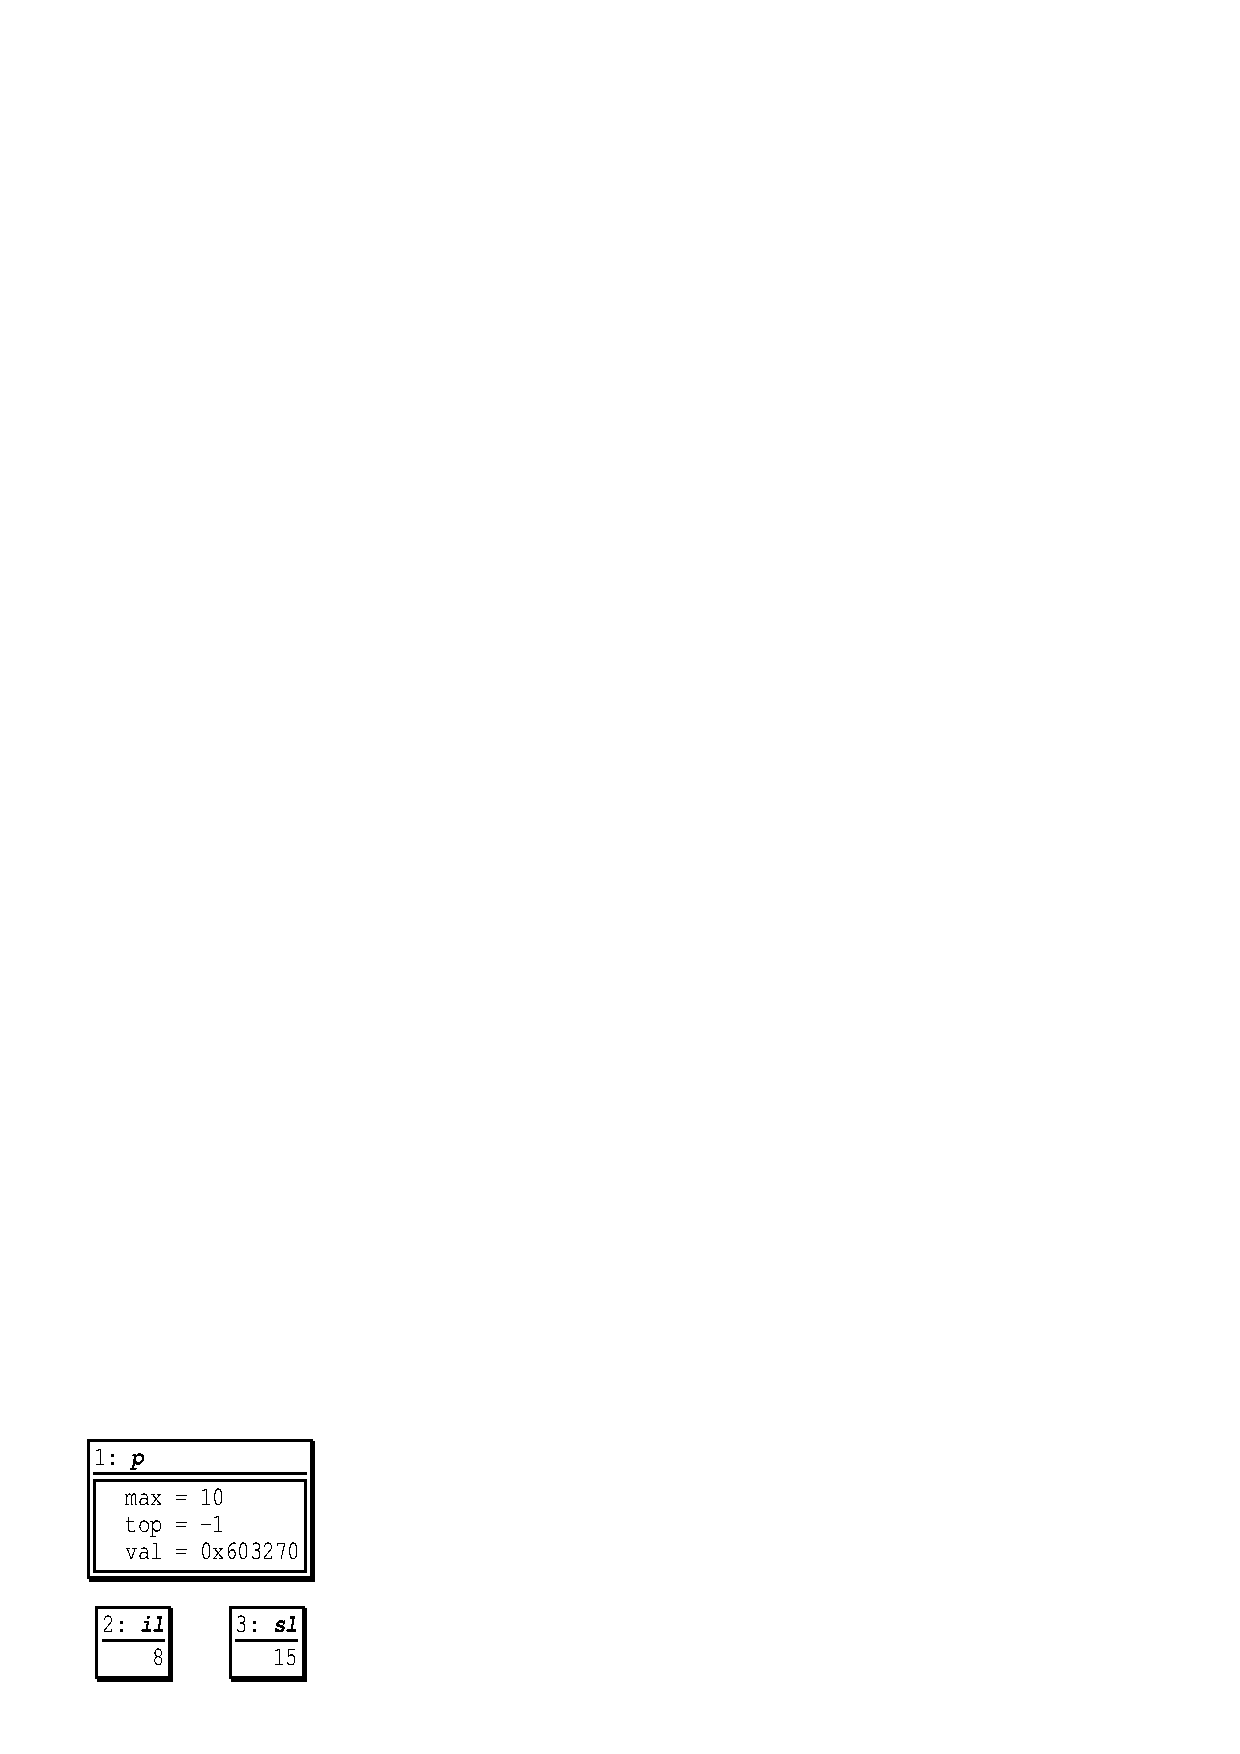
\includegraphics[width=3cm,clip=true,trim=1cm 1cm 15cm 24cm]{../tests/ddd_graph/ddd_4_11}
			\subcaption{Fin, après avoir dépilé 7}
		\end{subfigure}
	  \caption{Test n°4 -- Aperçu de la pile dans \texttt{ddd}}
	\end{figure}

\newpage
\subsection{Bonne utilisation de la mémoire}
	Pour vérifier la bonne libération de la mémoire, nous avons utilisé \texttt{valgrind} avec le programme seul. La fonction \texttt{main}, lorsqu'elle ne reçoit pas d'argument, lance un petit test sur les deux versions de la fonction \texttt{truc}, ainsi qu'un test sur la pile (initialiser, empiler jusqu'à ce que la pile soit remplie/dépiler jusqu'à ce qu'elle soit vide, libérer). Aucun bloc de mémoire n'est perdu, le retour texte de valgrind est présenté en figure \ref{fig:valgrind}.
	\begin{figure}[H]
	  \inputminted[frame=single,label=Resultat Valgrind]{text}{../tests/valgrind_test}
	  \caption{Passage dans l'outil \texttt{valgrind}}
	  \label{fig:valgrind}
	\end{figure}
